A wireless charger drives an alternating current through a flat coil ($L = \LzO$ without a phone), in series with a capacitor. It works at the resonance frequency, $f_0 = \fzO$, where the impedance is smallest and the current largest. The graph shows the impedance without a phone (dashed) and with a phone on the pad (solid): the ferrite sheet in the phone changes the inductance of the coil.

\begin{center}
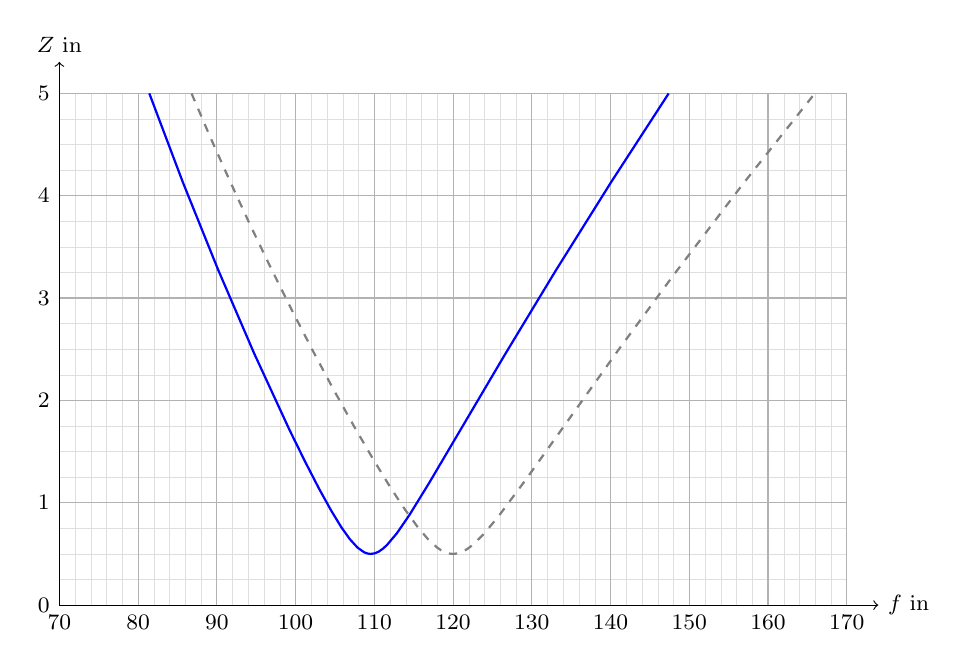
\begin{tikzpicture}[font=\footnotesize]
 \draw[gray!25, very thin] (0.200,0) -- (0.200,6.500) (0.400,0) -- (0.400,6.500) (0.600,0) -- (0.600,6.500) (0.800,0) -- (0.800,6.500) (1.200,0) -- (1.200,6.500) (1.400,0) -- (1.400,6.500) (1.600,0) -- (1.600,6.500) (1.800,0) -- (1.800,6.500) (2.200,0) -- (2.200,6.500) (2.400,0) -- (2.400,6.500) (2.600,0) -- (2.600,6.500) (2.800,0) -- (2.800,6.500) (3.200,0) -- (3.200,6.500) (3.400,0) -- (3.400,6.500) (3.600,0) -- (3.600,6.500) (3.800,0) -- (3.800,6.500) (4.200,0) -- (4.200,6.500) (4.400,0) -- (4.400,6.500) (4.600,0) -- (4.600,6.500) (4.800,0) -- (4.800,6.500) (5.200,0) -- (5.200,6.500) (5.400,0) -- (5.400,6.500) (5.600,0) -- (5.600,6.500) (5.800,0) -- (5.800,6.500) (6.200,0) -- (6.200,6.500) (6.400,0) -- (6.400,6.500) (6.600,0) -- (6.600,6.500) (6.800,0) -- (6.800,6.500) (7.200,0) -- (7.200,6.500) (7.400,0) -- (7.400,6.500) (7.600,0) -- (7.600,6.500) (7.800,0) -- (7.800,6.500) (8.200,0) -- (8.200,6.500) (8.400,0) -- (8.400,6.500) (8.600,0) -- (8.600,6.500) (8.800,0) -- (8.800,6.500) (9.200,0) -- (9.200,6.500) (9.400,0) -- (9.400,6.500) (9.600,0) -- (9.600,6.500) (9.800,0) -- (9.800,6.500);
 \draw[gray!25, very thin] (0,0.325) -- (10.000,0.325) (0,0.650) -- (10.000,0.650) (0,0.975) -- (10.000,0.975) (0,1.625) -- (10.000,1.625) (0,1.950) -- (10.000,1.950) (0,2.275) -- (10.000,2.275) (0,2.925) -- (10.000,2.925) (0,3.250) -- (10.000,3.250) (0,3.575) -- (10.000,3.575) (0,4.225) -- (10.000,4.225) (0,4.550) -- (10.000,4.550) (0,4.875) -- (10.000,4.875) (0,5.525) -- (10.000,5.525) (0,5.850) -- (10.000,5.850) (0,6.175) -- (10.000,6.175);
 \draw[gray!60, thin] (0.000,0) -- (0.000,6.500) (1.000,0) -- (1.000,6.500) (2.000,0) -- (2.000,6.500) (3.000,0) -- (3.000,6.500) (4.000,0) -- (4.000,6.500) (5.000,0) -- (5.000,6.500) (6.000,0) -- (6.000,6.500) (7.000,0) -- (7.000,6.500) (8.000,0) -- (8.000,6.500) (9.000,0) -- (9.000,6.500) (10.000,0) -- (10.000,6.500);
 \draw[gray!60, thin] (0,0.000) -- (10.000,0.000) (0,1.300) -- (10.000,1.300) (0,2.600) -- (10.000,2.600) (0,3.900) -- (10.000,3.900) (0,5.200) -- (10.000,5.200) (0,6.500) -- (10.000,6.500);
 \node[below] at (0.000,0) {70};
 \node[below] at (1.000,0) {80};
 \node[below] at (2.000,0) {90};
 \node[below] at (3.000,0) {100};
 \node[below] at (4.000,0) {110};
 \node[below] at (5.000,0) {120};
 \node[below] at (6.000,0) {130};
 \node[below] at (7.000,0) {140};
 \node[below] at (8.000,0) {150};
 \node[below] at (9.000,0) {160};
 \node[below] at (10.000,0) {170};
 \node[left] at (0,0.000) {0};
 \node[left] at (0,1.300) {1};
 \node[left] at (0,2.600) {2};
 \node[left] at (0,3.900) {3};
 \node[left] at (0,5.200) {4};
 \node[left] at (0,6.500) {5};
 \draw[->] (0,0) -- (10.400,0) node[right] {$f$ in \si{\kilo\hertz}};
 \draw[->] (0,0) -- (0,6.900) node[above] {$Z$ in \si{\ohm}};
 \draw[thick, gray, dashed] plot coordinates {(1.679,6.497) (1.920,5.935) (2.167,5.383) (2.420,4.835) (2.679,4.296) (2.944,3.763) (3.211,3.245) (3.479,2.743) (3.741,2.273) (3.979,1.863) (4.196,1.508) (4.384,1.221) (4.546,0.998) (4.679,0.840) (4.796,0.732) (4.849,0.696) (4.901,0.670) (4.951,0.655) (5.001,0.650) (5.058,0.657) (5.116,0.677) (5.178,0.711) (5.243,0.759) (5.389,0.902) (5.574,1.124) (5.916,1.583) (7.123,3.273) (7.805,4.198) (8.681,5.348) (9.595,6.500)};
 \draw[thick, blue] plot coordinates {(1.142,6.499) (1.569,5.368) (2.014,4.264) (2.474,3.196) (2.924,2.222) (3.121,1.822) (3.297,1.480) (3.451,1.202) (3.582,0.987) (3.691,0.835) (3.786,0.731) (3.872,0.670) (3.914,0.655) (3.954,0.650) (4.002,0.657) (4.052,0.677) (4.104,0.712) (4.159,0.762) (4.286,0.912) (4.446,1.145) (4.697,1.553) (5.653,3.173) (6.298,4.239) (7.006,5.370) (7.738,6.498)};
\end{tikzpicture}
\end{center}

\begin{abcliste}
\abc What is the capacitance $C$?
\abc Where is the minimum with the phone?
\abc What is the inductance $L_1$ of the coil with the phone?
\end{abcliste}
